%
%You can keep the 12pt font size, or go to 11pt or (default) 10pt
% Do NOT go any larger than 12pt font size for submission
%
%If you want to edit a printed copy, you may want to add draft mode
% (as in \documentclass[draft,conference,12pt]{IEEEtran})
% This adds space between the lines providing easier editing markup
%
%For more details see 
% http://ras.papercept.net/conferences/support/files/IEEEtran_HOWTO.pdf
%
\documentclass[conference,12pt, ]{IEEEtran}
\usepackage[margin=1truein]{geometry}
\usepackage{cite}
\usepackage{graphicx}
\usepackage{algorithmic}
\usepackage{url}
\usepackage{flushend}
\usepackage{listings}
\usepackage{setspace}
\usepackage{times}

% correct bad hyphenation here
\hyphenation{op-tical net-works semi-conduc-tor}

\begin{document}


\title{Avoiding General Purpose Microcontrollers For Multirotor Autonomous Flight }

\author{
	\IEEEauthorblockN{Innocent Niyibizi}
  \IEEEauthorblockA{Computer Science Department\\Missouri University of Science and Technology\\Rolla, MO 65409\\
  Email: iniyibizi@mst.edu}
}


% make the title area
\maketitle

\doublespace
\begin{abstract}
As the world continues to develop, more and more problems arise that can be solved with the use of advanced software systems. These problems can be things such as navigating an unfamiliar environment or surveying known environments after disaster strikes. To accomplish these goals, months of R\&D is poured into specific problems and how to solve them with the current technological advances. 
\end{abstract}

\section{Introduction}
Technological advances happen all throughout the country and in many different disciplines. The one that is the most notable is "drone" technology. The technology spans from tiny, harmless pocket drones to the stealthy, yet deadly, USA Military Unmanned Aerial Vehicles. With the development of drone hardware and software, we're now able to move from human operated flights into flights that are all in the control of the vehicles. The ability to have these vehicles operate without human intervention will open a number of doors for modern problems to be solved with modern solutions. This is where organizations, such as The International Aerial Robotics Comptetition (IARC), comes into play.\\
The IARC is an competition that strives to push the boundaries of aerial flights and problem solving. Each year year they have so called missions for what they consider to be the most important area of focus. These missions can range from autonomously flying around a given area to autonomously herding Roomba vacuum cleaners in a 25mx25m gym onto one side. Each mission will have its fair share of restrictions and technological advances that must be had before the mission can be completed. \\
These missions are geared towards college teams/organizations to take their shot solving the issue which opens the door for creative. A design team on campus, The Multirotor Robot Design Team(MRR) is one such team and has been tackling this since 2016. They have gone through many microcontrollers, specifically flight boards, and have found the feasibility of each one for the given task.

\section{History}
MRR has been in the autonomous flight field since the very beginning but they could not have gotten there without the short comings and the lessons learned along the way. One of the most important things learned along the way, is the need for the right sensors and flight board for autonomous based tasks. The team experimented with two microcontrollers before settling with one that really suites their needs. Each one has its unique features and feasibility to the challenge at hand: Fly autonomously in an indoor environment with limited sensor input.

\subsection{APM Flight Board}
The APM flight board was the very first board that the team used in their attempts in autonomous flight. Figure 1 outlines the design of the board itself along with the pinout. This particular board, APM 2.X has since been discontinued but is still capable of running firmware up to Arducopter, an open source flight firmware, 3.3 \cite{apm_board}. This line of boards is also based around the AVR CPUs. Because of the discontinuation of the APM board, the team was unable to achieve the tasks at hand. 

\subsection{Arduino}
Like many robotics based projects, the Arduino was an obvious choice to try to attempt the challenge of restricted, autonomous flight. Figure 2 outlines the pinout for the Arduino Mega and it was used as the first attempt at creating a custom flight controller. The overall goal was to use the Arduino as both the onboard computer as well as the flight controller. The onboard computer portion of the Arduino would be used to write the code necessary to fly and then send which ever commands are necessary in the given moment to the autopilot \cite{on_board}

\subsection{Pixhawk}
The Pixhawk is the real star of the show and is where much of the focus will be since it is the most updated flight controller and has the most capabilities to complete the challenges at hand. The Pixhawk leverages the power of a different microporcessor from revision to revision, the one of interest for now is the Cortex -M4. Figure 3 depicts the organization of the Cortex-M4 along side the Pixhawk Cube with its carrier board.

\section{The Microcontrollers That Could}
\subsection{APM Flight Board: Captain}
\begin{figure}
	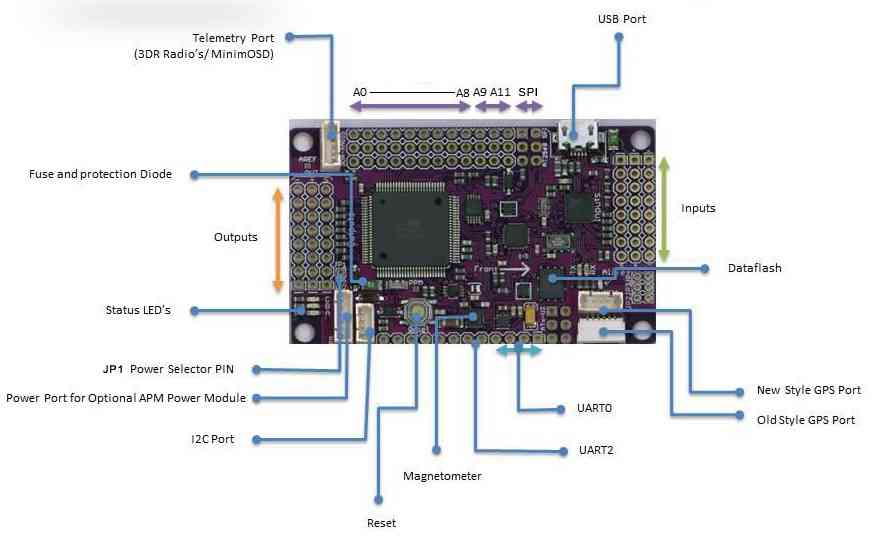
\includegraphics[scale=0.40]{apm2.jpg}
	\caption {Layout of APM2.5 Flight Controller}
\end{figure}
During the early development years of MRR, they were experimenting with the possibilty of building a drone from scratch. This meant developing the frame, the propellers and motors, and more importantly the electronics for the drone. Since the first year wasn't focused on the autonomy of the challenge, the team was in search of a flight board to control the motors and other accessories such as the camera gimbal. 
\subsubsection{Features}
The APM Board comes with a plethora of options and feature and some of the more notable ones include: Telemetry, GPS, I2c, analog input pins, digital output pins. \cite{apm_board}\\
These features each have their unique features but since this is supposed to designed to be a flight board, it has the other features such as an IMU and barometer. 
\subsubsection{Use Cases}
For this flight board the two use cases are manual and aided, autonomous flight. The manual flight is built into the flight board, as all it takes is a few simple processes such as calibrating each sensor and the electronic speed controllers (ESC). The aided, autonomous flight is also a use case but is dependent on having a GPS, which would need to be added externally. It is feasible to achieve some autonomous features with an onboard computer but, without certain sensors, it will be limited in its abilities. 
\subsubsection{Task Feasibility}
The APM board is a great board for flying custom built drones manually, but autonomously is another story. As MRR advanced from year to year, more and more solid ideas to achieve autonomous flight were developed.

\subsection{ATmega1280: Arduino Mega }
\begin{figure}
	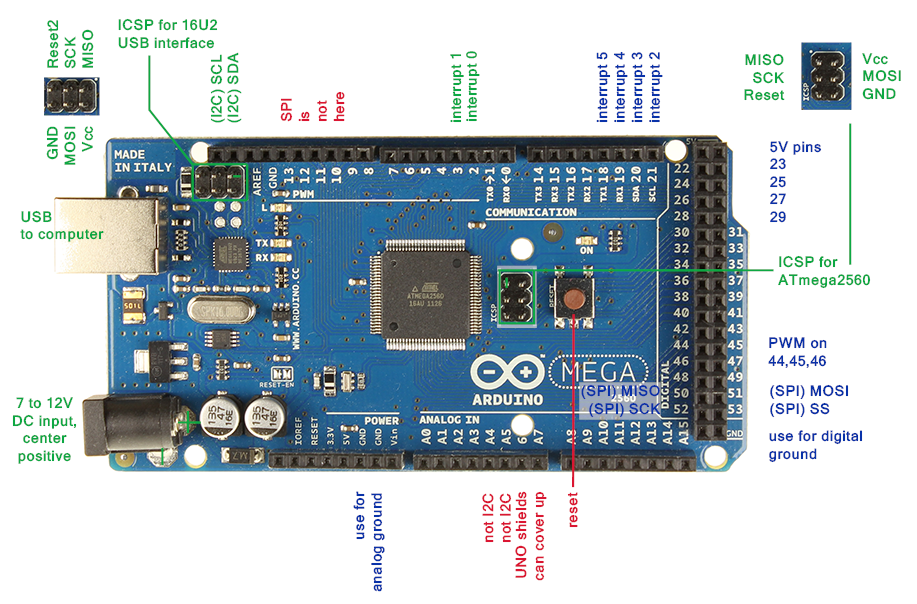
\includegraphics[scale=0.25]{mega.png}
	\caption {Layout of Arduino Mega  Microcontroller}
\end{figure}
As MRR started to enter their first attempts at achieving fully autonomous flight, the idea was given that an Arduino would be a good board to use. This idea was presented in the form that the Arduino would act as the flight board, controlling the motors and acting as a bridge for other auxiliary sensors, as well as acting as the companion computer which will run the autonomous code. 
\subsubsection{Features}
Because of the versatility of the Arduino Mega, it was the perfect choice for this first attempt. The Mega includes the following inputs and outputs built off of the ATmega1280:  Serial, PWM, and I2c.\cite{arduino} \\
The Mega also features a suite for writing C based code to interface with the controller and I/O at a higher level, though not as high of a level as the Pixhawk which will be discussed later. 
\subsubsection{Use Cases}
There are many articles and papers that exist which point the creation of custom drones to use some sort of Arduino as the flight controller. While this is perfect for manual flight, it is much more difficult for fully autonomous flight. For an arduino to function as a flight controller it will utilize the serial ports to interface with the transmitter and receiver while also utilizing the PWM features of the board to control the motors of the frame. 
\subsubsection{Task Feasibility}
The Arduino family is known for being a family of microcontrollers that are perfect for general purpose use cases and more specific use cases if given the time to really adapt them. However, it is not the best option for having the board be an companion computer as well as the full flight board. It has more than enough communication protocols to communicate with any sensors connected, via I2c or serial, but with the SRAM size of $8KB$ and a clock speed of $16Mhz$ \cite{arduino}, that is not nearly enough processing power available to sustain fully autonomous flight. Manually flight is possible, based solely on converting the digital signals to analog PWM values, and doing some telemetry work on the sensor data. 

\subsection{Cortex-M4: PixHawk 2 (The Cube)}
\begin{figure}
	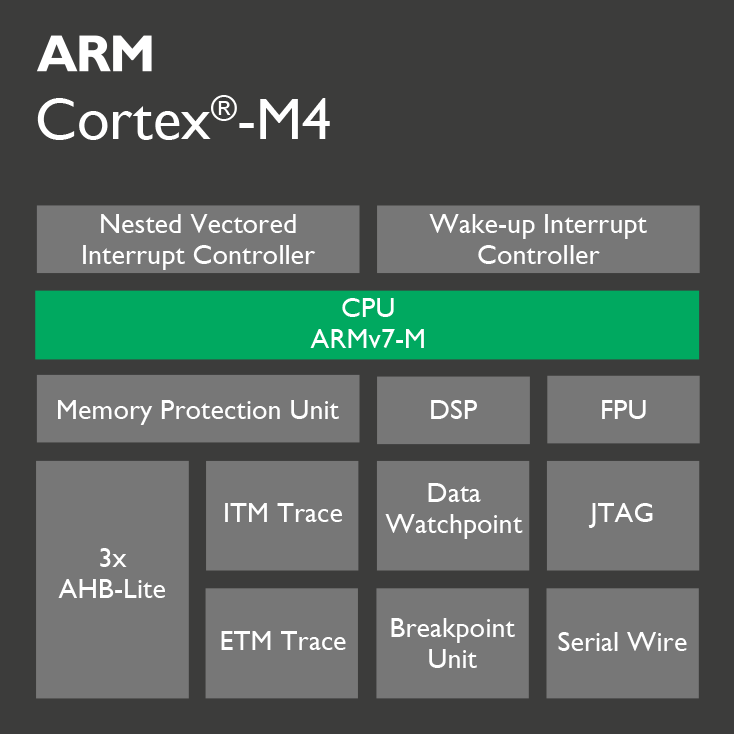
\includegraphics[scale=0.12]{cortex.png}
	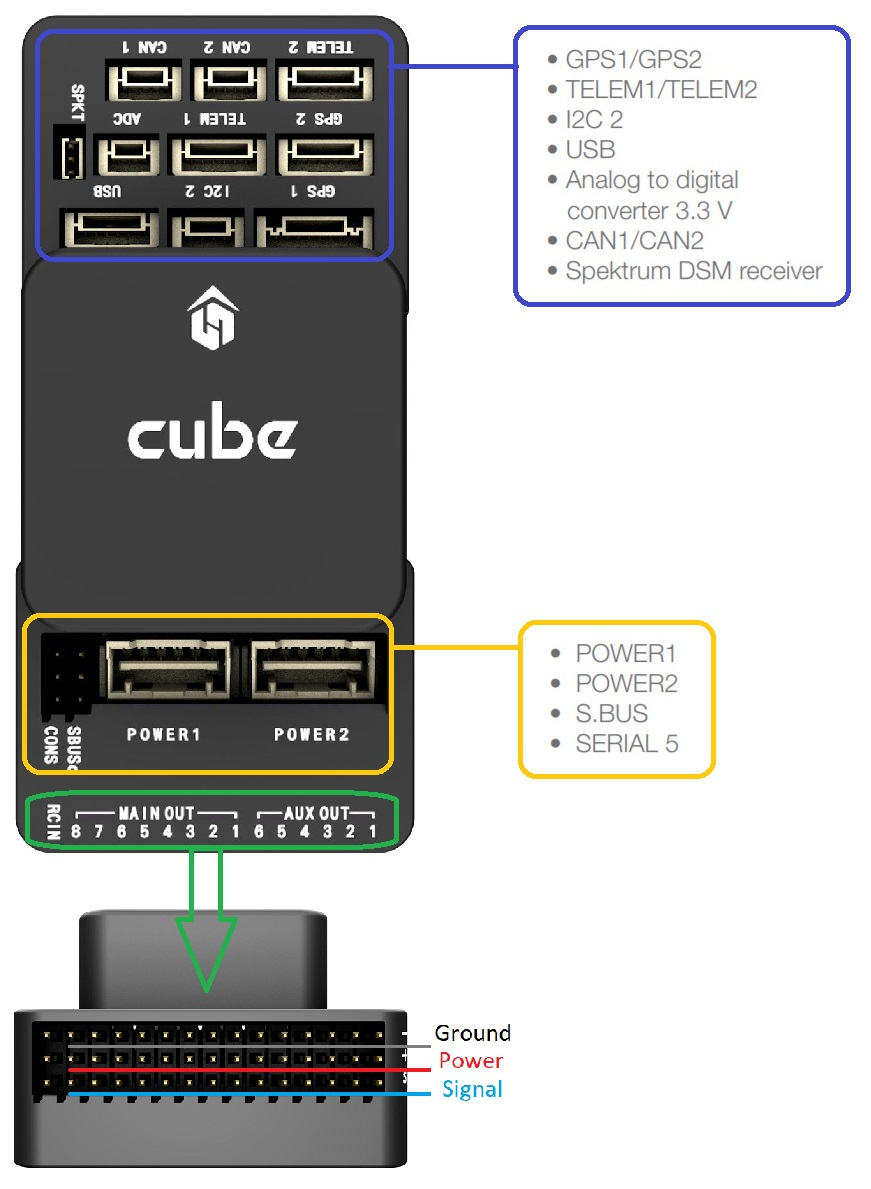
\includegraphics[scale=0.25]{cube.jpg}
	\caption{Cortex-M4 and Pixhawk 2(The Cube)}
\end{figure}
In the open source flight community, the Pixhawk is the unofficial champion. This family of flight boards sport a plethora of I/O as well as the processing power and specs to tackle any tasks thrown at them. Figure 3 shows one of the newest additions to the Pixhawk family, The Pixhawk 2: Cube, and the microcontroller that does all the heavy lifting, the Cortex-M4. Because of it's capabilities this was a clear choice for MRR to use to develop their autonomous systems. 

\subsubsection{Features}
There is a reason that the Pixhawk family is the unofficial king of the open source flight controller family and that is for the many features that they have to offer. These features include, but are not limited to: IMU, 14 PWM / Servo outputs, $256 KB RAM$, clock speed of $168 MHz$, UART, and I2c. The most important feature is to flash a pre-compiled firmware that is specialized for the given use case to make programming and usage more diverse. 
\subsubsection{Use Cases}
With the ability to flash custom, pre-compiled firmwares onto the Pixhawk, this opens the doors to many applications and use cases. The main focus for this paper is the Ardupilot line of firmwares which include: Copter, Rover, and Plane. The Pixhawk is able to abstract the specific functionality and give high level development for the most advanced autonomous features. Along with autonomous use cases, manual operation is built in and with the default senors and ability to add more, the manual flight is some of the most stable and feature rich. 
\subsubsection{Task Feasibility}
One of the main purposes of the Pixhawk is to make flight operations as painless as possible by allowing as much plug and play as the market and hardware allows. With this, each and every sensor imaginable has some value to the flight operations. Some of the more notable sensors are rangefinders and optical flow sensors using the I2c protocol. These two sensors combined with the default flight modes allow multirotors sporting the Pixhawk to be an unstoppable force. The Pixhawk also features many forms of telemetry and high level programming for fully autonomous flight, given some sort of companion computer and other external cameras or mapping devices.


\section{Conclusion}
Tie everything back together and explain why the pixhawk, being a specialized flight board is necessary for the task at hand.

\clearpage
  \begin{thebibliography}{999}

  \bibitem{apm_board}  APM Board  {\em [Online]. Available: \url{http://ardupilot.org/copter/docs/common-apm25-and-26-overview.html#common-apm25-and-26-overview}} [Accessed: 11-Mar-2019].

  \bibitem{arduino} Arduino Mega{\em [Online]. Available: \url{https://www.arduino.cc/en/Main/arduinoBoardMega/}} [Accessed: 11-Mar-2019]

  \bibitem{optical_flow} OpenCV Otical Flow {\em [Online]. Available: \url{https://docs.opencv.org/3.3.1/d7/d8b/tutorial_py_lucas_kanade.html}} [Accessed: 11-Mar-2019]

\bibitem{pixhawk_cube} Pixhawk Cube {\em [Online]. Available: \url{https://docs.px4.io/en/flight_controller/pixhawk-2.html}} [Accessed: 11-Mar-2019]

\bibitem{on_board} Companion Computers {\em [Online]. Available: \url{http://python.dronekit.io/develop/companion-computers.html#supported-companion-computers}} [Accessed: 11-Mar-2019]

  \end{thebibliography}
\end{document}

